\subsection{Backward Stepwise Selection}

The second method applied is the dual of the previous one, i.e. \textit{Backward Stepwise Selection}. The model obtained is shown in figure \Fig~\ref{fig:BackwardModelSummary}.
\begin{figure}[h]
	\centering
	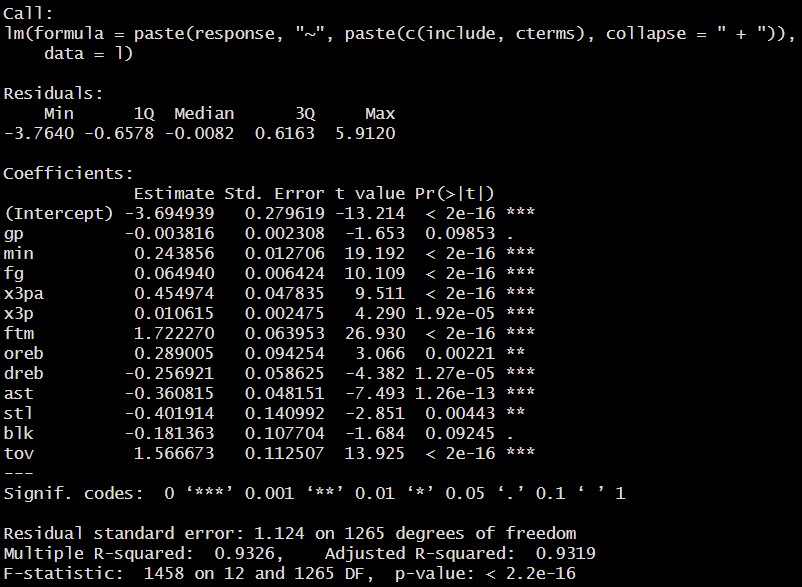
\includegraphics[width=0.4\linewidth]{ImageFiles/Regression/Backward/BackwardModelSummary}
	\caption{Backward Stepwise Selection Output Model.}
	\label{fig:BackwardModelSummary}
\end{figure}